\documentclass[12pt, letterpaper]{article}
\usepackage{graphicx} % Required for inserting images
\graphicspath{{./figures/}}
\usepackage{listings} % Required for inserting code
\lstset{inputpath=./src/}
\usepackage{xcolor} % Required for formatting code

\title{Assignment 2 - LaTeX Write Up}
\author{Connor Fleischman}
\date{November 1, 2024}

\definecolor{background}{rgb}{0.95,0.95,0.92}
\definecolor{codegreen}{rgb}{0,0.6,0}
\definecolor{codegray}{rgb}{0.5,0.5,0.5}
\definecolor{codepurple}{rgb}{0.58,0,0.82}
\definecolor{magenta}{rgb}{1,0,1}
\definecolor{backcolour}{rgb}{0.95,0.95,0.92}
\definecolor{keywordcolor}{rgb}{0.82,0.1,0.26}

\lstdefinestyle{mystyle}{
   backgroundcolor=\color{background},   
   commentstyle=\color{codegreen},
   keywordstyle=\color{keywordcolor}\bfseries,
   numberstyle=\tiny\color{codegray},
   stringstyle=\color{codepurple},
   basicstyle=\ttfamily\small,
   frame=single, 
   rulecolor=\color{codegray},
   breakatwhitespace=false,         
   breaklines=true,                 
   captionpos=b,                    
   keepspaces=true,                 
   numbers=left,                    
   numbersep=10pt, 
   showspaces=false,                
   showstringspaces=false,
   showtabs=false,                  
   tabsize=4,
   emph={int,char,double,float,unsigned}, 
   emphstyle={\color{blue}},
}

\lstset{style=mystyle}

\begin{document}
\maketitle
\begin{center}
   
\includegraphics[width=120mm,scale=0.5]{MaristSeal.png}
\end{center}
\newpage

%%%%%%%%%%%%%%%%%%%%%%%%%%%%%%%%%%%%%%%%%%%%%%%%%%%%%%%%%%%%%%%%%%%%%%%%%%%%%%%%%%%%%%%%%%%%%%%%%%%
\section{Assignment Results}
Assignment 2 was to perform different searches on the magic items text file provided in Assignment 1 for 42 random keys, picked from the magic items.

\subsection{Linear Search} \label{LinSch}
The first search to be performed was a linear search.
This searching method takes a key and sequentially picks through each magic item, comparing the current item to the key, until the key is found.
After implementing this in C++ and ensuring that my algorithm is correct, 10 tests were performed and their data recorded below.
\begin{center}
   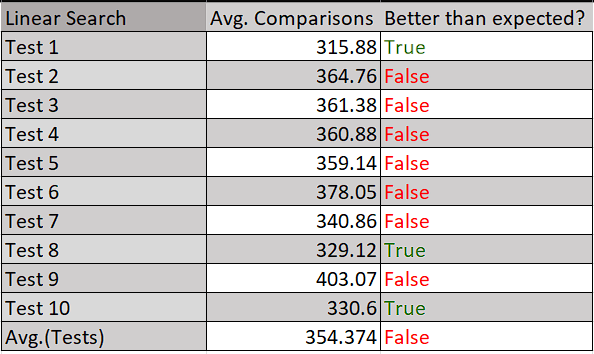
\includegraphics[width=120mm,scale=0.5]{LinSearch.png}
\end{center}
This table diagrams the average time each test took to find all 42 keys in magic items. 
It also depicts how efficient the algorithm was.
Before we continue, it is important clarify a few prerequisites.
\begin{center}
   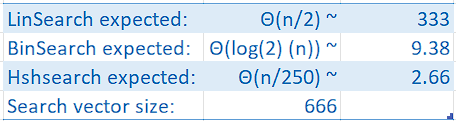
\includegraphics[width=120mm,scale=0.5]{Prerequisites.png}
\end{center}
With these in mind, the 'Better than expected?' column now has a basis to compare to.
So over the performed tests, the data shows that only 30\% of all searches, for the 42 keys, performed were more efficient than the expected value.
Not an amazing result for my code, however only 10 tests were performed, who's to say that if 100 tests took place it wouldn't spread to 50\%.

\subsection{Binary Search} \label{BinSch}
A binary search was the next task to conquer.
This search takes a key and the middle value of the sorted magic items.
Compares if the middle item is or is not the key, if it is not, then it compares if the middle item is larger or smaller than the key.
Finally if the key is larger than the middle item, the search is ran again on the half greater than the middle.
Otherwise the key is smaller and the search is ran on the half smaller than the key.
\begin{center}
   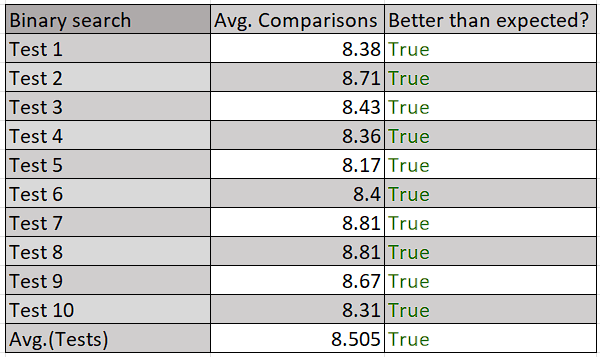
\includegraphics[width=120mm,scale=0.5]{BinSearch.png}
\end{center}
The same 10 tests were performed for binary search with each test's keys being the same for each numbered test.
Meaning, the keys used for test one in linear search were the same keys used for binary search (and for hash searching).
\newline
\indent As shown above, the binary searching algorithm I implemented was quite efficient.
But the same logic applied to linear search applies here, although 100\% of tests were more efficient than the average case, does not mean that with more testing it can't be inefficient.

\subsection{Hash Table Search} \label{HshTblSch}
The last search assigned was to take the magic items, create a hash table of 250 buckets, populate it with the items, and search for the keys using the hash table.
A hash table is a 2-dimensional table where each value in the table has its own table of values.
\newline
\indent So in relation to the problem, the hash table stores each magic item in a bucket corresponding to its ASCII value.
This allows a search to narrow down the possible answers much more quickly than linear and binary search, leading to a much more efficient algorithm.
\begin{center}
   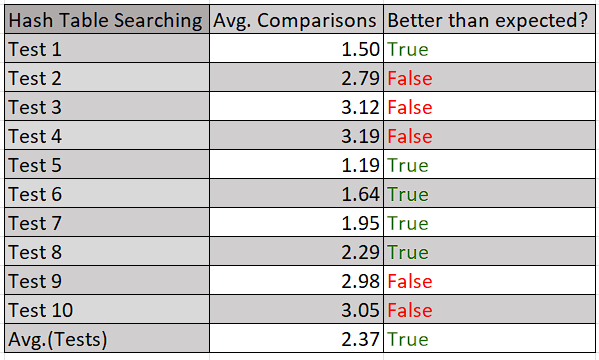
\includegraphics[width=120mm,scale=0.5]{HshSearch.png}
\end{center}
After conducting the same 10 tests, using the same 42 keys per tests, the data has shown that 50\% of tests performed were above the average efficiency of a hash search.
It also shows how efficient hash searching is compared to the other searching algorithms above.
It would be interesting to see if the average of all tests would fall below the expected threshold if more tests were performed.

%%%%%%%%%%%%%%%%%%%%%%%%%%%%%%%%%%%%%%%%%%%%%%%%%%%%%%%%%%%%%%%%%%%%%%%%%%%%%%%%%%%%%%%%%%%%%%%%%%%
\section{Code Breakdown - main.cpp}
My code consists of three C++ documents. 
A 'main.cpp' file housing the majority of the computations, and two assistive files, 'sortItems.h' and 'buildHashTable.h'.
These files are woven together through 'main.cpp' so that when executed it prints out the results of the searches to the console.
These files are in the './Assignment 2/src' folder.

\subsection{Breakdown - main()} \label{Main}
Our program begins through the main function below.
Do not worry if this seems complex, we will break it down piece by piece.
\lstinputlisting[language=C++, firstline=104, lastline=135]{main.cpp}
When the executable is ran a vector of strings called \textit{keys} is declared and instantiated as sort.first().
This comes from the 'sortItems.h' file which returns a pair of vectors, for more detail see section \ref{SrtItm}.
Then \textit{sorted} is instantiated as sort.second(), from 'sortItems.h', for more detail see section \ref{SrtItm}.
\newline
\indent A linear search is then performed for each key in keys using the sorted magic items.
Next, the average comparisons is calculated and produced for that search on each key.
After a binary search is used for the same keys as before to search through magic items.
Again, the program calculates and produces the average number of comparisons for a key based off the 42 keys.
\newline
\indent Finally, the code clears the sorted list and creates a hash table from 'buildHashTable.h' using createTable().
The same search is performed for the same 42 keys as prior, but instead of searching through the magic items, the program uses a hash table populated with the magic items.
Then the average comparisons is found and output and the comparison count is reset to 0 and keys and the hash table are all cleared.

%%%%%%%%%%%%%%%%%%%%%%%%%%%%%%%%%%%%%%%%%%%%%%%%%%%%%%%%%%%%%%%%%%%%%%%%%%%%%%%%%%%%%%%%%%%%%%%%%%%
\section{Code Breakdown - Linear \& Binary Search}
Assignment 2 required us to perform a linear search and a binary search, using 42 randomly chosen keys, on the sorted list of magic items.

\subsection{Breakdown - sortItems.h} \label{SrtItm}
The main function in section \ref{Main} uses a function from 'sortItems.h'.
Specifically, it uses the pair of return values given from the sort() method.
It sets a vector of strings called \textit{keys} to sort().first, and \textit{sorted}, which was defined in section \ref{Prereq}, as sort().second afterwards.
\newline
\lstinputlisting[language=C++, firstline=13, lastline=48]{sortItems.h}
As we can see on line 35, sort().first is keys and sort().second is the insertionSort() function.
\textit{Keys} is defined as a vector of strings which, after randomly selecting a starting value within the bounds of the data, we store the next 42 values as keys.
This is done on lines 27-33.
\newline
\indent Insertion sort is defined on line 1 and has a return value of a vector of strings.
Insertion sort takes the unsorted magic items, written to a vector of strings, sorts it using an insertion sort, and returns it to sort().second.
This is why we set 'keys = sort().first' (ln 3, sec \ref{Main}) and 'sorted = sort().second' (ln 4, sec \ref{Main}).
Finally in the sort() function we read the file 'magicItems.txt' into a vector of strings called \textit{lines} for manipulation.

\subsection{Breakdown - linearSearch()} \label{LinSchCde}
Below is my implementation of a linear search algorithm which takes a searching vector and a key.
This function sequentially searches each item in the vector until it finds the key, incrementing a counter for each comparison made.
Then when the value is found it will output the number of comparisons performed to find it and add that to the comparison count.
\newline
\indent If the value is not found, then it will not increment the comparison count and simply return that the value was not found after being compared to every other value.
\lstinputlisting[language=C++, firstline=21, lastline=40]{main.cpp}
A linear search algorithm should, on average, find its key $\frac{n}{2}$ times where \textit{n} is the number of values being searched through, in this case 666.
So we expect the search to return its key after an average of 333 ($\frac{666}{2}$) comparisons.
As seen above, my code does linearly search through every item in magic items until the key is found, therefore my algorithm is of $\frac{n}{2}$ efficiency on average. 

\subsection{Breakdown - binarySearch()} \label{BinSchCde}
Listed below is the binary search algorithm I created. 
This function will take the middle value of the sorted magic items and compare it to the key.
After checking for equality, if not equal, then it will compare if the key is greater than or less than the middle value.
Depending on if the key is larger or smaller, the binary search will then recursively call itself on whatever half the key belongs to until the value is found at the middle.
\newline
\indent This method is inherently more efficient than a linear search as the amount of values to be search through decreases by half each time the function recurs. 
\lstinputlisting[language=C++, firstline=42, lastline=72]{main.cpp}
Binary searching, as mentioned, is more efficient than linear searching.
And rightfully so since linearly searching through a graph is slower than repeatedly cutting it in half.
The average efficiency of a binary search is $\log_2 n$, where \textit{n} is 666 (the size of the search vector).
\newline
\indent Therefore, when we calculate $log_2 (666)$ we find that the expected number of comparisons required to find a key is 9.38.
Comparing this to my code we see that the algorithm does recursively call itself on the half that the key belongs to, making it $\log_2 n$.
So this implementation of binary search is effective.

%%%%%%%%%%%%%%%%%%%%%%%%%%%%%%%%%%%%%%%%%%%%%%%%%%%%%%%%%%%%%%%%%%%%%%%%%%%%%%%%%%%%%%%%%%%%%%%%%%%
\section{Code Breakdown - Hash Table Searching}
Assignment 2 also required us to build a hash table with a bucket size of 250. 
Sort the magic items, load them into these buckets, and perform searches for the keys using this table.

\subsection{Breakdown - buildHashTable.h} \label{BldHshTbl}
The file 'buildHashTable.h' is ran through the createTable() function on line 29.
In this function, a vector of strings called magic items is made and populated with the magic items from 'magicItems.txt' (ln 31 \& 32).
Then the hash table is created with a bucket size of 250 (ln 33). 
Afterwards, the hash table is populated with the magic items, this creates each bucket and fills it with its respective items (ln 34).
Finally the table is returned (ln 35).
\lstinputlisting[language=C++, firstline=10, lastline=49]{buildHashTable.h}
This code was influenced from the 'Hashing\_cpp.txt' file (from labouseur.com) as many it's methods are similar.
The makeHashCode() function turns a given item into the sum of each character's ASCII value.
It then returns the remainder of that value divided by the number of buckets in the hash table to get the value of the item's bucket.
\newline
\indent The buildTable() function takes a list of items and the unpopulated hash table and populates it.
Specifically, the function will take every item in the list of items, create its hash code for it, then push that code into the hash table (making it's bucket).

\subsection{Breakdown - searchItem()} \label{HshSchCde}
The function searchItem(), in 'main.cpp' is used to search for a specific item in the hash table.
It is called for each key in the list of keys and afterwards, the average number of comparisons for all the key's searches is computed.
\lstinputlisting[language=C++, firstline=83, lastline=102]{main.cpp}
As we can see, on line 5 the hash code value of the key is calculated.
Then we check, for every item in the bucket corresponding to the hash value of the key, if the value is not equal to the key, check the next value.
\newline
\indent If we find the value then it will print to the console the number of comparisons it took to find the value.
That number is then added to the running comparison count. 
If the value is not found after searching through the bucket, then it prints that the value was not found to the console.
Comparison count is incremented by 0, so nothing changes.

%%%%%%%%%%%%%%%%%%%%%%%%%%%%%%%%%%%%%%%%%%%%%%%%%%%%%%%%%%%%%%%%%%%%%%%%%%%%%%%%%%%%%%%%%%%%%%%%%%%
\section{Misc.} \label{Misc}
Below is all remaining code.
Anything not mentioned before this point is defined and explained below.
\subsection{averageComparisons()} \label{AvgComp}
Here we are calculating the average number of comparisons needed to find every key in the sorted, or hashed, data set.
\lstinputlisting[language=C++, firstline=74, lastline=81]{main.cpp}
To round to two decimal places, as specified in the Assignment 2 instructions, we must use a fixed precision floating point number.
To find the average of the comparisons we use a globally scoped variable called comparisonCount defined in section \ref{Prereq}.
With this we divide it by the total number of keys, defined in section \ref{SrtItm} on line 3.
This gives us the average which is then output to the console to two decimal places.
Then the comparison count is reset to 0 for the next search.

\subsection{main.cpp - Prerequisites} \label{Prereq}
\lstinputlisting[language=C++, firstline=10, lastline=19]{main.cpp}
Beginning 'main.cpp' we include 'buildHashTable.h' and 'sortItems.h' as well as 'iostream' and 'iomanip'.
These allow us to use functions like createTable() and sort.first() or .second() for our algorithms.
They also allow for use of console output and floating point number precision respectively. 
We also use the std namespace as to not have to add 'std::\_' to the code.
\newline
\newline
Globally scoped variables:
\newline
\indent comparisonCount - the total number of comparisons for a search
\newline
\indent sorted - a vector of strings to store the sorted magic items
\newline
\indent hashTable - a vector of vectors of strings, or a vector of buckets of strings

\subsection{sortItems.h - Prerequisites} \label{SrtItmGV}
\lstinputlisting[language=C++, firstline=1, lastline=10]{sortItems.h}
In 'sortItems.h' we make use of importing 'fstream' for reading the 'magicItems.txt' file to a vector.
Also, 'vector' is used for vector manipulation, and 'algorithm' to use the "swap" instruction.
The std namespace is still used for simplicity.
\newline
\newline
Globally scoped variables:
\newline
\indent lines - where magic items will be written to
\newline
\indent keys - the 42 keys to be searched for
\newline
\indent KEYS\_SIZE - specifies that we will be searching for 42 keys
\newline
\indent file - the file to be read from when making lines
\newpage

\subsection{buildHashTable.h - Prerequisites} \label{BldHshTblGV}
\lstinputlisting[language=C++, firstline=1, lastline=7]{buildHashTable.h}
The 'buildHashTable.h' file uses two include statements, one for 'fstream' which, same as before, is used to read the file to a vector.
The second is 'vector' which allows us to control the data in a specified vector.
Again, the std namespace is used.
\newline
\newline
Globally scoped variables:
\newline
\indent HASH\_TABLE\_SIZE - the number of buckets used in the hash table

%%%%%%%%%%%%%%%%%%%%%%%%%%%%%%%%%%%%%%%%%%%%%%%%%%%%%%%%%%%%%%%%%%%%%%%%%%%%%%%%%%%%%%%%%%%%%%%%%%%
\section{Final Thoughts}
This assignment was, at least for myself, more straightforwards and easier to comprehend than Assignment 1.
This could be because I find myself more well versed in C++ and LaTeX as the semester continues, or maybe its because I actually learned something.
Regardless, this assignment was very enjoyable to code, and even debug. 
Although C++ can be weird, especially when it comes to memory allocation, it is a fun language to learn and I look forwards to the upcoming assignments.
\end{document}